% !TEX TS-program = LuaLaTeX

\documentclass[12pt]{article}

\usepackage[urw-garamond]{mathdesign}
\usepackage[T1]{fontenc}
\usepackage{fontawesome}
\usepackage{enumitem}
\usepackage{scrextend}
\usepackage{etaremune}
\usepackage[rightcaption]{sidecap}
 
\usepackage{graphicx} %package to manage images 

% use http link for email
\usepackage[colorlinks = true,
          linkcolor = MidnightBlue,
           urlcolor  = MidnightBlue,
           citecolor = MidnightBlue,
           anchorcolor = MidnightBlue]{hyperref}            
            
%allow formula formatting
\usepackage{amsmath}
\DeclareMathAlphabet\mathbfcal{OMS}{cmsy}{b}{n}
\usepackage{comment}

%title positon
\usepackage{titling} %fix title
\setlength{\droptitle}{-6em}   % Move up the title 

%change section title font size
\usepackage{titlesec}
\titleformat{\section}
  {\normalfont\fontsize{12}{15}}{\thesection}{1em}{}[{\titlerule[0.5pt]}]
  
\titleformat{\subsection}
  {\normalfont\fontsize{12}{13}}{\thesection}{1em}{}

% change page margin and cancel identation
\usepackage[top=0.8in, bottom=0.8in, left=0.7in, right=0.7in]{geometry} 
\setlength{\parindent}{0pt}

%allow modifying section titles 
\usepackage[dvipsnames]{xcolor}

% Make lists without bullets
\renewenvironment{itemize}{
  \begin{list}{}{
    \setlength{\leftmargin}{1.5em}
    \setlength{\itemsep}{0in}
  }
}{
  \end{list}
}


\begin{document}

    \begin{flushleft}
    \textbf{
    {\huge C}{\Large HROM} {\huge N}{\Large ET--Chromatin-based cellular phenotype classification}}\\
     \hspace*{4mm} Caleb Lareau, BST 290 Midterm\\
     \hspace*{4mm} Prepared for 5 November 2016
         \end{flushleft}

%\begin{addmargin}[6.5mm]{4mm}   
\section{\textbf{{\Large A}{\small BSTRACT }}}
Recent advances in stem cell technology have enabled the isolation of induced pluripotent stem cells from committed cell lineages, providing a powerful framework for novel therapeutics and investigating cell-fate decisions. To assess factors relevant to inducing pluripotency, bioinformatics approaches have been proposed using transcriptional regulatory networks with some success. However, as transcriptional data can fail to clearly distinguish cellular phenotypes, we hypothesized that these methodological advancements could be improved. Thus, we introduce ChromNet, a novel computational approach that assigns cellular phenotypes to new samples using a reference panel of chromatin accessibility from ATAC-Seq data. We apply ChromNet to induced pluripotent cell states from blood and identify novel transcription factors associated with development cascades and cell-fate decision. 

 \section{\textbf{{\Large I}{\small NTRODUCTION}}}
The discovery of induced pluripotent stem cells (iPSC) from committed cell lineages has revolutionized cell biology.\textsuperscript{1} In particular, the ability to induce pluripotent cell states from committed lineages has afforded a remarkable experimental program to discern systems associated with cellular differentiation from embryonic and pluriopotent stem cells. To facilitate the identification of factors relevant to the generation of iPSCs, bioinformatics approaches such as CellNet\textsuperscript{2} have been developed that use a background of committed tissue types and infer properties of new samples based on this background. The authors of CellNet\textsuperscript{2} use gene regulatory networks from microarray data to classify samples and identify new transcription factors based on the importance of the factor in a transcription network, which helped with the induction of pluripotency from multiple committed cell lines. \newline \newline While CellNet provided one option for identifying factors that may assist in identifying factors related to iPSCs, the method has a couple of short comings. First, the authors use only 26 microarray samples when establishing their background. As microarray samples take 10,000 or more cells to generate data and are an outdated technology, the backbone of CellNet is incompatible with modern bioinformatics analyses. Moreover, identifying cellular phenotypes through transcriptomic data isn't as effective as profiling phenotypes from open chromatin data\textsuperscript{3} from assays such as ATAC-Seq.\textsuperscript{4} Table 1 shows the relative cluster purities of hematopoietic samples directly comparing chromatin profiles and transcriptomic profiles.\textsuperscript{4}

\begin{table}[h]
\begin{center}
  \begin{tabular}{ | c | c | c | c | c | }
    \hline
    \multicolumn{5}{ |c| }{Cluster purities of hematopoietic cells} \\ \hline
    Data Type & RNA-Seq & ATAC-Seq & Promoter ATAC & Distal Enhancer ATAC\\ \hline
    Cluster Purity & 0.776 & 0.857 & 0.675 & 0.909 \\ \hline 
  \end{tabular}
  \caption{Cluster purities of hematopoietic cells from a previous manuscript.\textsuperscript{3} While these cellular phenotypes are closely related, variable open chromatin at distal enhancer regions enables a strong separation of these phenotypes in the samples considered. Transcriptomic data as well as open chromatin at promoters were less effective in distinguishing cellular phenotypes in unsupervised clustering. }
\end{center}
\end{table} \newpage

Additionally, as only 26 samples are used in ChromNet, the background data would ideally incorporate more tissues and samples than what previously exists in a new tool. Figure 1 shows the growth of ATAC-Seq, which we propose would be a better data basis than microarray due to the exponential growth noted, more than 1,000 samples profiles across mouse and human, and the low input (500 cells).\textsuperscript{4}

\begin{SCfigure}[0.5][h]
\caption{Growth of ATAC-Seq. Since the original description of the protocol in 2013, more than 2,000 samples are publicly available on GEO in both mouse and human. Additionally, the growth of this assay is increasing exponentially. New assays added each year are noted in the bar graphs stratified by organism. These numbers only consider bulk samples that could be downloaded from GEO determined by HTML scrubbing, but additional samples may be available through other public resources and in single cells. }
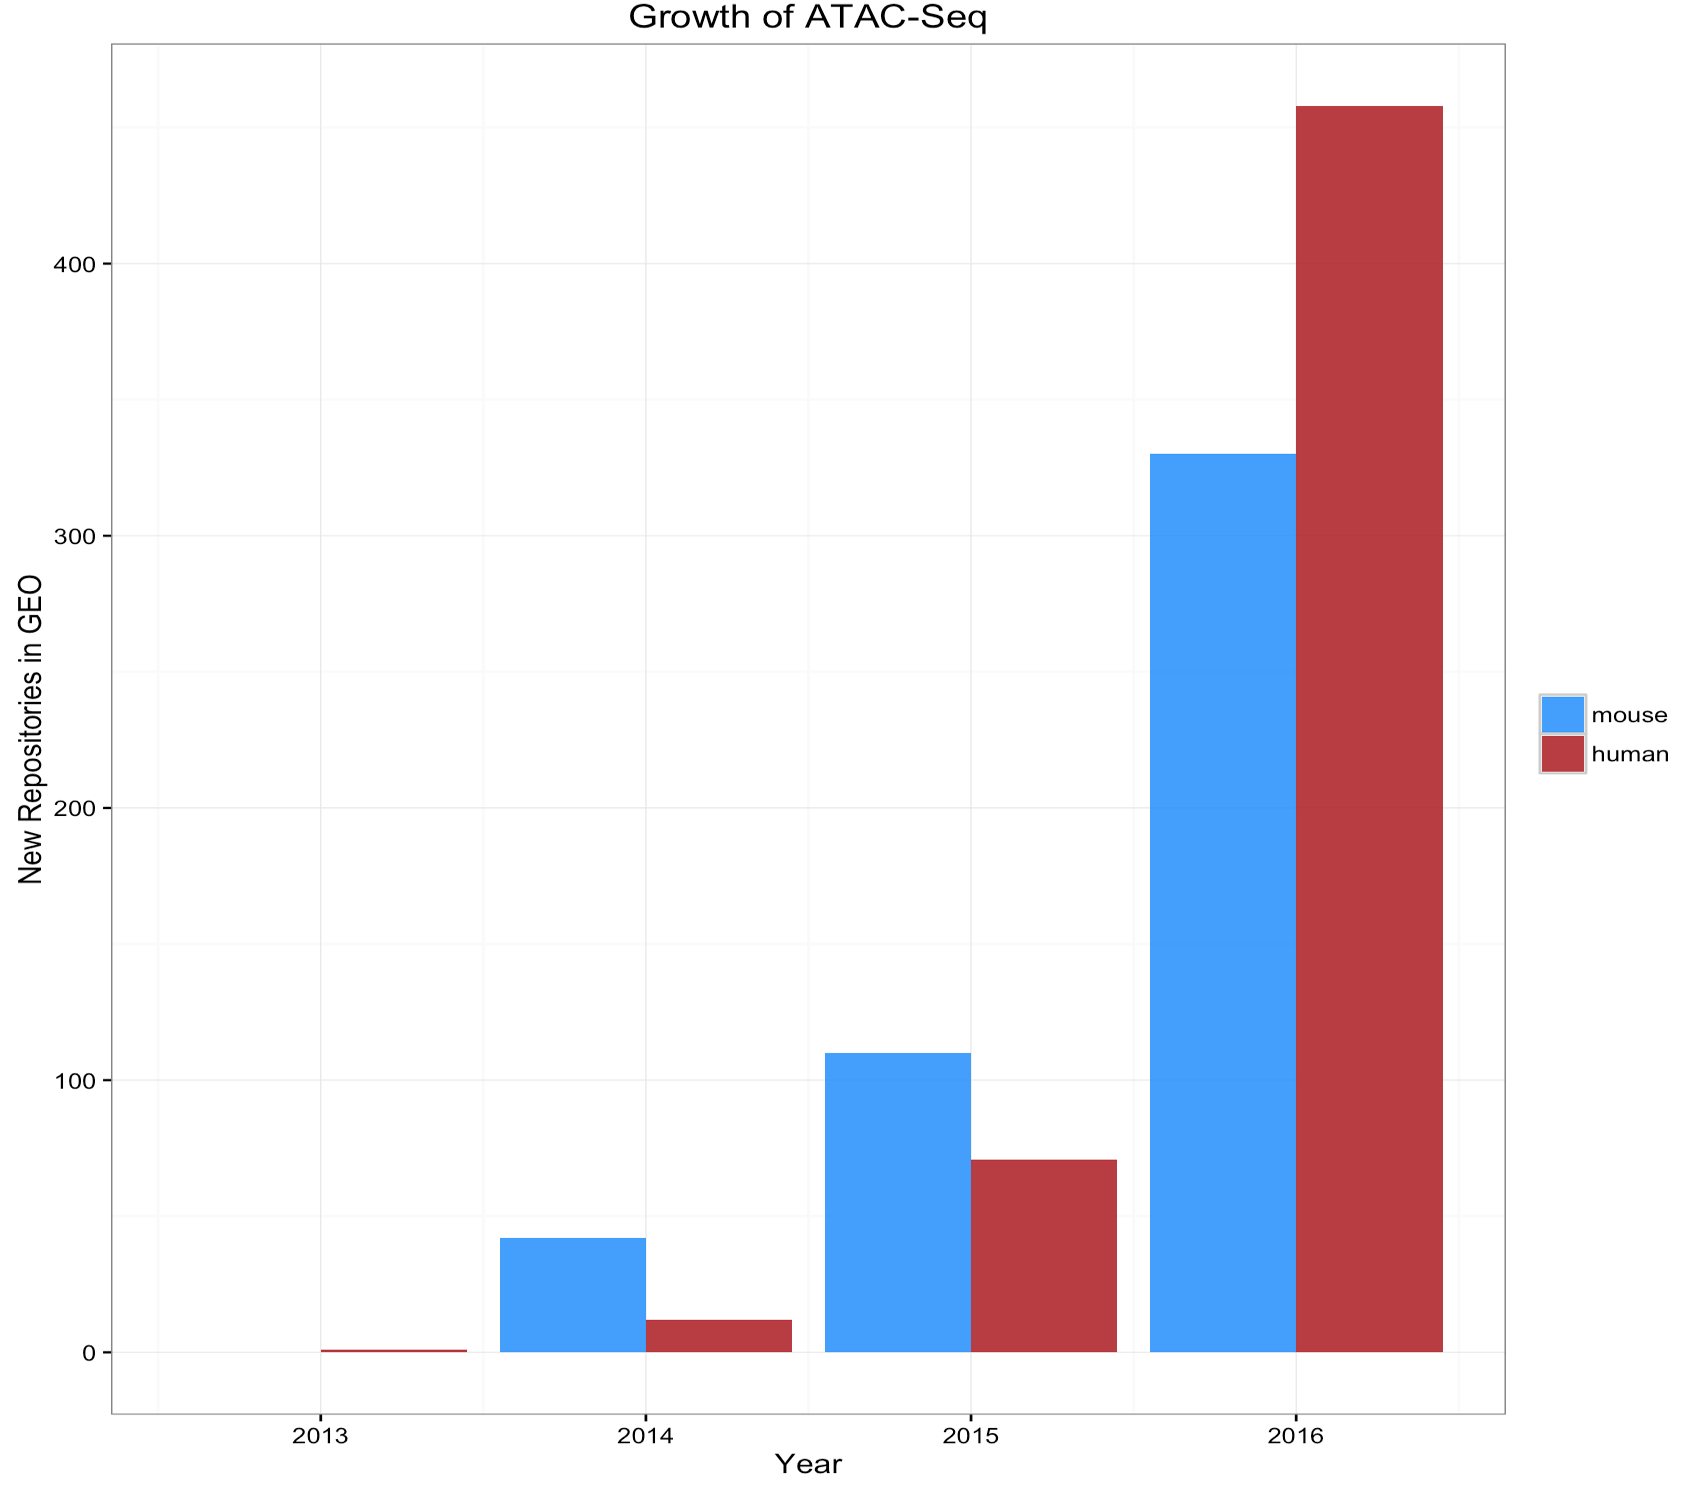
\includegraphics[scale=0.45]{atac_growth.png}
\end{SCfigure}

Finally, the identification of transcription factors potentially responsible for the maintenance and direction of cell differentiation is a key feature of CellNet. As the total open chromatin supporting a motif is a better proxy for the importance of a factor than the mRNA expression of the factor,\textsuperscript{3} we suggest that using chromatin data will identify more useful transcriptional regulators that can drive variance in cellular phenotypes associated with iPSC. Taken together, we introduce ChromNet, an open source computational platform, that infers cellular phenotypes based on open chromatin from hundreds of ATAC-Seq profiles and recommends transcription factors pertinent to iPSC experiments. To demonstrate the efficacy of ChromNet, we identify novel transcription regulator factors previously unidentified in CellNet relevant to the induced pluripotency of fibroblasts as previously described.\textsuperscript{2} \newpage

 \section{\textbf{{\Large M}{\small ETHODS}}}
 
\textbf{Data Collection} \newline
 Noting the wealth of publicly available ATAC-Seq data from GEO (Figure 1), we will first perform an HTML parsing to determine all relevant sequencing read archives associated with ATAC-Seq samples and all meta-data. We will collect this raw sequencing data and descriptions and commonly preprocess each sample using established methods.\textsuperscript{4} In general, preprocessing of ATAC-Seq data requires 1) linker removal, 2) deduplication, 3) alignment, and 4) peak calling.  \newline

\textbf{Analysis Methods} \newline
(brief) While CellNet\textsuperscript{2} uses a rather extensive algorithm to identify gene regulatory subnetworks to classify unknown samples, I first propose to do principle component clustering using simple Euclidean distances as a classifying mechanism. More advanced avenues include Random Forest and other machine learning approaches. \newline 

\textbf{iPSC Culture Experiments} \newline
We will collaborate with external labs who can perform the cell culture experiments to generate iPSCs and then perform ATAC-Seq on these cells before feeding the chromatin profile data from these experiments into our model for classification and identification of transcription factors that would drive differentiation. New ATAC-Seq data will be generated on these iPSC stem cells. 

 \section{\textbf{{\Large R}{\small ESULTS}}}
(brief) Data analysis results \newline
We can generate quality control measures associated with each sample to filter out for experiments of poor quality. High quality samples will be systematically processed in principle component space and in machine learning applications to reduce dimensionality and identify factors specific to those cellular phenotypes.  \newline

(brief) Validation results  \newline
Similarly generate ATAC QC metrics to validate the new ATAC experiment. Then, assign similarity based on an existing profile. Expect to see some mixture of the previous mature state (e.g. fibroblast), pluripotent states (e.g. CD34+), and the new mature state. 

 \section{\textbf{{\Large D}{\small ISCUSSION}}}
(brief) Interpretation: Primarily will focus on ensuring that similar cell types (e.g. in blood) cluster together relative to other distal tissues. Using identified factors from ChromNet hopefully helped in the conversion of iPSC cell types. \newline \newline Ultimately, ChromNet provides a useful tool for identifying factors associated with cellular differentiation such as those shown in Figure 2. We hope to populate this map more using this bioinformatics technology coupled with the iPSC experimental system. 

\begin{center}
\begin{figure}[h]
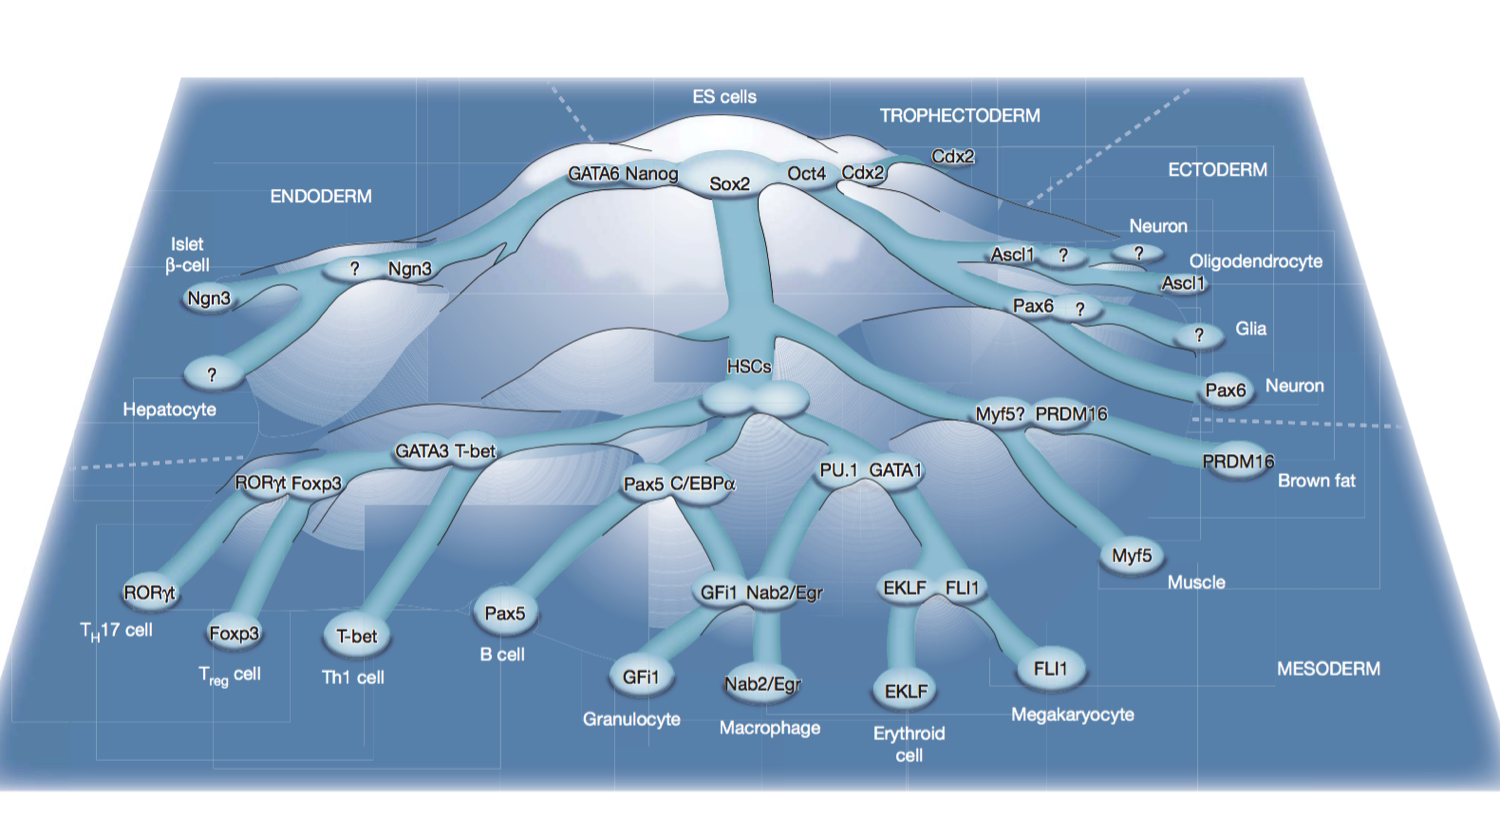
\includegraphics[width=0.85\paperwidth]{tf_landscape.png}
\caption{Transcription factors in a cascading landscape of cell states. Differentiated cell types are represented as basins whereas unstable theoretical cell states correspond to ridges and slopes in the landscape. The latter types of cells are observed infrequently during development and thus unlikely to correspond to observable cell types. Characterizing this landscape and the factors associated in moving from one type to another is vital for characterizing epigenetic plasticity. Image reproduced from a previous manuscript.\textsuperscript{5}}
\end{figure}
\end{center}


 \section{\textbf{{\Large R}{\small EFERENCES}}}
 \textsuperscript{1} Yu, Junying, et al. "Induced pluripotent stem cell lines derived from human somatic cells." Science 318.5858 (2007): 1917-1920. \newline
 \textsuperscript{2} Cahan, Patrick, et al. "CellNet: network biology applied to stem cell engineering." Cell 158.4 (2014): 903-915. \newline 
  \textsuperscript{3} Corces, M. Ryan, et al. "Lineage-specific and single-cell chromatin accessibility charts human hematopoiesis and leukemia evolution." Nature Genetics (2016). \newline 
 \textsuperscript{4} Buenrostro, Jason D., et al. "Transposition of native chromatin for fast and sensitive epigenomic profiling of open chromatin, DNA-binding proteins and nucleosome position." Nature methods 10.12 (2013): 1213-1218. \newline 
 \textsuperscript{5} Graf, Thomas, and Tariq Enver. "Forcing cells to change lineages." Nature 462.7273 (2009): 587-594. \newline
%\end{addmargin}
\end{document}

